\subsection{Personalize the data for each user}

So far we have seen different parameters to evaluate the relevant data at a general level. In this section, we will focus on the specific personal level.
Each user has a unique personal situation, so we have to find a way to adapt and personalize the data, to provide both general and individually specific information.
For example, if I was the user, my defining characteristics such as where I live,
my health status, family situation, etc can help us.\\

In many cases, we will not be able to fully customize, but we can look for common points in subgroups of
user. From this point we have to study the different cases that can be given and make a selection of those that are
more common.\\

The key question we need to consider in order to be able to personalize the information, is how can the data be related at a specific time, in a specific place to meet specific needs of the
user as an individual.

\subsubsection*{Suggested strategies} 

\begin{itemize}
  \item We should study how the data will help the user or user-subgroups as we mention in the section \textit{3.3 Know your user} and from this point, make it more specific. In this way
    we go from obtaining relevant data in a general way to be relevant in a personal way.
  \item We have to think about the
    particular user, and find a way to extract the results that are specifically adapted to them in a particular
    moment and place.
\end{itemize}

\subsubsection*{In the context of Aire Guru \ldots}

 We are all interested in the pollution that surrounds us, since it affects our health. The webtool
 Aire Guru has been designed to specialize in this area. For those people who are especially sensitive to air pollution, Aire Guru shows the air pollution with respect to the six most common medical conditions that
 are affected by air pollutants.
 
\begin{figure}[ht]
  \centering
  \subfigure[EPOC]
    {\includegraphics[width=3.5cm  ]{filter_epoc}}
  \hfill
  \subfigure [Asthma]
      {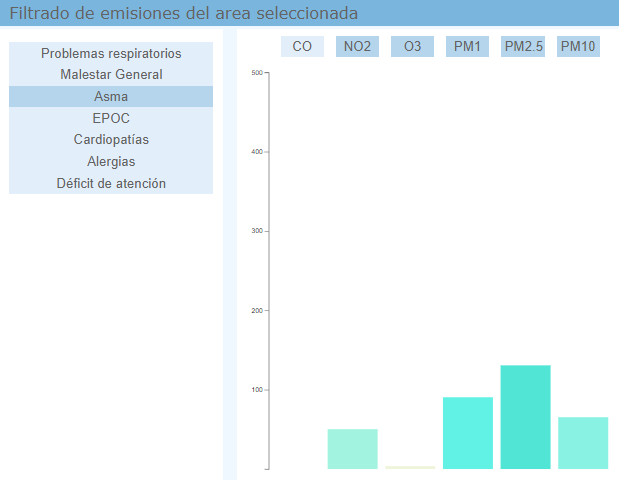
\includegraphics[width=3.5cm]{filter_asthma}}
  \hfill
  \subfigure[Allergies]
    {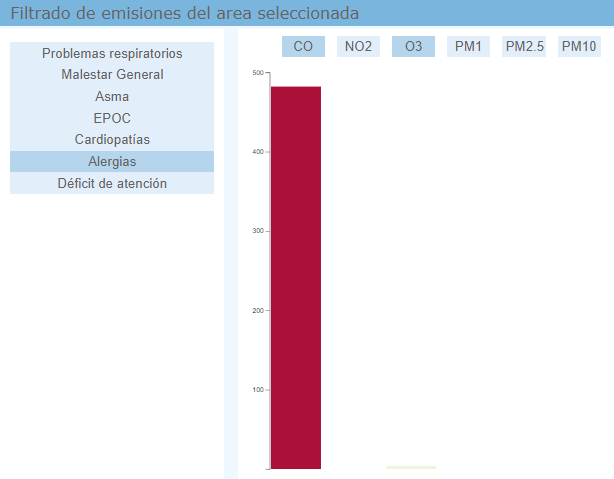
\includegraphics[width=3.5cm]{filter_allergies}}
  \caption{Medical Condition Filter}
\end{figure}

In the \textit{Figure X.X} we see, in each case, for each medical condition, a subset of pollutants which most influence each condition is shown.\\
  
The answer to the key question, how can the data be related to a specific time and place, leads us to
implementation of a personal history of exposure to pollution. That is, to know at all times what pollution
a user is subject to and where the exposure happened.\\

For this, it is essential to read the user's position. By matching the users location and the coordinates provided by the original dataset, we can find the level of exposure to pollutants.
If the user gives us his permission to store this data, we can show them their personalized history.

\begin{figure}[ht]
  \centering 
  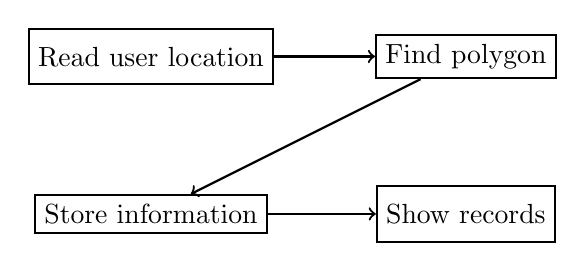
\begin{tikzpicture}[thick]
    \node[draw,rectangle,minimum size=20] (a) {Read user location};
    \node[draw,rectangle,minimum size=6,right of= a, node distance=4cm] (b) {Find polygon};
    \node[draw,rectangle,minimum size=5,below of= a, node distance=2cm] (c) {Store information};
    \node[draw,rectangle,minimum size=20,right of=c, node distance=4cm] (d) {Show records};
    \draw[->] (a) to (b);
    \draw[->,] (b) to (c);
    \draw[->] (c) to (d);
  \end{tikzpicture}
  \caption{Collecting user location}
\end{figure}

This functionality is Aire Guru most powerful tool. Other platforms require user-level measurement devices, ie the user must carry
a portable measurement station that monitors the different pollutants. \\

\begin{figure}[ht]
  \centering
  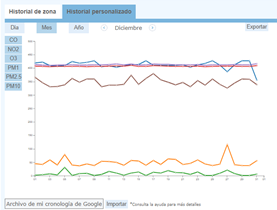
\includegraphics[width=8cm]{importedDataDecember}
  \caption{Personal Records. December}
\end{figure}

It is possible that the user may have started to use the application and not yet have any available data.
To deal with this, we offer the possibility of importing the Google location history, enabling the user to be able to visualize
exposure to pollution since the beginning of 2018 even if they have not been using the webtool for  all of that period.\\

We will have to take into account that in order to read the user's position and store their data, we must
have their explicit permission. We must implement mechanisms that provide us with the necessary security to safeguard our users data. The measures taken will be explained later.

\begin{itemize}
  \item The user has specialized functionalities
  \item Unique functionality, the user is able to see the pollution to which he has been exposed since 2018 even if they have not been using the tool since that time.
  \item The filtering function of the medical condition is not self-selected, because the functionality
        is available to all users. The map could show the AQI with respect to the
        pollutants that the user has preselected, but this can de-visualize the information if it is not
        clearly indicated to the user that the map does not take into account all relevant pollutants.
\end{itemize}
